%version of 06-18-19

\chapter{``DOING'' MATHEMATICS: \\
A Toolkit for Mathematical Reasoning}
\label{ch:doingmath}


\begin{quote}
{\em \ldots where a Mathematical reasoning can be had, it's as great
  folly to make use of any other, as to grope for a thing in a dark,
  when you have a candle standing by you.} \\
\hspace*{2in} John Arburthnot, {\it Of the Laws of Chance}, 1692
\end{quote}

\noindent
Mathematics can be viewed as a discipline that crafts formal models of
real phenomena or structures and then uses the models to reason
rigorously about reality.  This is a daunting charter for the neophyte
who aspires to ``do'' mathematics.  How does one observe and isolate
the features of a real phenomenon within a formal model?  What, in
fact {\em is} a {\em formal} model.  Once has has such a model, how
does one use it to reason {\em rigorously} about the piece of reality
that the model is intended to capture?

This chapter represents our attempt to answer the preceding daunting
questions.  Of course, details and examples will await the technical
chapters of this text.  What we present here merely lays the
foundation by providing intuition and motivation and examples.  This
chapter ``amuses the palate''\footnote{\ldots in the sense of the
  French {\em amuse-bouche}.}~in preparation for the introductory
mathematical repast that we offer the reader.  Before we present the
hors d'oeuvres that we hope will entice the reader, we ``set the
table'' for our feast.


Somewhat surprising to the non-mathematician, a large portion of
``doing'' mathematics, the widely touted ``queen of the
sciences''\footnote{See, e.g., Wolfgang Sartorius von Waltershausen,
  {\it Gauss zum Ged\"{a}chtniss} (1856).}, is {\em
  pattern-matching}---albeit of a monumentally sophisticated variety.
Mathematicians are trained to understand pieces of reality to a depth
that allows them to understand how apparently unrelated concepts $A$
and $B$ can be conceptualized via the same {\em abstract
  representation}, and to analyze (computational, in our bailiwick)
advantages to exploiting such representations.  It may be useful to
the reader to keep the ``mathematics-as-pattern-matching'' metaphor in
mind while reading (from) this book, all the better to enjoy the many
instances of pattern-matching that populate its pages.

This text is devoted to the practice of mathematics within the world
of computing.  By means of plentiful examples, we hope to convince the
reader of the importance of mathematics in one's quest to master the
technology and the methodology of computing.  By means of extensive
explanations---we often prove the same fact many times, from multiple,
orthogonal vantage points---we provide the reader tools to recognize
mathematical aspects of computational settings and phenomena and
technology, and we provide guidelines for using those tools
effectively.

We begin with two motivational aphorisms.

\medskip

\noindent {\sc Regarding mathematical models}.

%\medskip

\noindent
{\it Entia non sunt multiplicanda praeter necessitatem.}

\hfill {\small William of Occam (14th cent.)} \index{William of Occam}
\index{Occam's Razor}\index{The Principle of Parsimony}

\smallskip

\noindent
{\it Occam's Razor}, or {\it The Principle of Parsimony} urges the
reader to ``Keep every (philosophical) argument as simple as
possible''.  This quest for simplicity is an essential component of
quality as one seeks mathematical models of computational phenomena
and as one reasons about one's models.

\medskip

\noindent {\sc Regarding mathematical argumentation}.

\noindent
{\it I mean the word proof not in the sense of the lawyers, who set
  two half proofs equal to a whole one, but in the sense of a
  mathematician, where ${1 \over 2}$ proof $= 0$, and it is demanded
  for proof that every doubt becomes impossible.}

\hfill {\small Carl Friedrich Gauss,\index{Gauss, Carl Friedrich}
  letter to Heinrich Wilhelm Matthias Olbers (14 May 1826)}

\smallskip

\noindent
Without being prescriptive regarding the form of the arguments that
mathematicians accept as ``proofs'', Gauss articulates the essential
required characteristic of such arguments.

\bigskip

The task of crafting mathematical models requires knowledge of the
domain being modeled, so we delegate this topic to the subject areas
that motivate the reader's interest in mathematics.

But the task of crafting mathematical arguments that are rigorous yet
accessible is {\em precisely} what we strive to accomplish with this
text.  Without further ado, let us begin our exploration into the
craft of mathematical reasoning.

\section{Rigorous Proofs: Theory vs.~Practice}
\label{sec:reasoning-via-proofs}


Contrary to the all-too-common view of mathematics as arcane strings
of symbols that must be manipulated in rigid ways, mathematics is a
vibrant, evolving system of thinking whose evolution is influenced by
the ever-changing objects that are being thought about and by the
ever-changing population that are doing the thinking.  That said,
mathematics does have its Cesium atom against whose internal
vibrations we can---{\em in principle}---measure any mathematical
argument.  Indeed, the quest for such a standard occupied much of the
early 19th century.

\bigskip

\noindent \fbox{
\begin{minipage}{0.95\textwidth}
We do not go back earlier than the 19th century in our quest for rigor
in mathematical proofs because formal notions of ``rigor'' are,
historically, a relatively recent phenomenon.  Indeed, many ``proofs''
predating the 19th century fall below the standard that we now expect
even of students---usually by failing to resolve---or even mention---
every crucial issue raised in a proferred argument.

\bigskip

Perhaps the most famous example of omitted details relates to the
famous ``last theorem'' of the great French polymath Pierre de Fermat.
\index{Fermat, Pierre de} During the 1630s, Fermat made (in Latin, of
course) the following claim in the margin of a copy of the classic
{\it Arithmetica}, by 3rd-century mathematician Diophantus:
\index{Diophantus}
\begin{quote}
{\it It is impossible to separate a cube into two cubes, or a fourth
  power into two fourth powers, or in general, any power higher than
  the second, into two like powers.  I have discovered a truly
  marvelous proof of this, which this margin is too narrow to contain.}

In modern parlance: \\
{\it There do not exist positive integers $a$, $b$, and $c$ such that
  $a^k + b^k = c^k$ for any positive integer $k >2$.}
\end{quote}
Fermat attributed the absence of details to the absence of room to
supply them in the margin.

\smallskip

It is, indeed, possible that the small margins in Fermat's copy of
{\it Arithmetica} were the only cause for his omitting a detailed
argument.  Subsequent history, though, suggests that the real cause
for the omission was the absence in the 17th century of the
mathematics needed to prove the theorem.  A complete proof of the
theorem was published only in 1995, by the English mathematician (Sir)
Andrew Wiles, \index{Wiles, Sir Andrew John} using highly novel
mathematics whose development occupies an entire issue of the journal
{\it Annals of Mathematics} \cite{Wiles95}.
\end{minipage}
}
\bigskip

The ultimate development of a ``Cesium atom'' for mathematical proofs
resulted from seminal philosophical developments by mathematical
logicians in the 19th century.  Not surprisingly, the length and
rigidity of style of these ultimate-standard proofs made them quite
unfriendly for humans to either craft or understand.  Just as we allow
a carpenter to use a tape measure rather than a scored platinum bar,
we allow humans to employ a human-palatable mode of argumentation in
all situations.  We turn now to a description of the mathematical
analogue of the Cesium atom that we aspire to and a discussion of the
mathematical analogue of the tape measure that we actually work with.


\subsection{Formalistic Proofs and Modern Proofs}
\label{sec:classical-v-modern-proofs}

This section is a rather informal discussion of rather formal topics.
The presentation here is introductory and motivational; it is expanded
and made rigorous in the remainder of the book.  The reader will find
in Section~\ref{sec:Propositional-logic} a rigorous presentation of
much of the coming material.


\subsubsection{Formalistic proofs, with an illustration}
\label{sec:formal-proof}

The purely formalistic view of mathematical discourse is devoid of
intuition or imagery.  Each discourse is just a sequence of
syntactically valid {\it statements}.  Certain designated statements
are {\em axioms}---meaning ``self-evident truths''.  There are also
{\em rules of inference}---formal rewriting rules---which enable one
to create new statements from sequences of pre-existing ones and to
append these new statements to the discourse.  Within this world:
\begin{itemize}
\item
A {\em proof} is a sequence of statements.
  \begin{itemize}
  \item
The first statement must be an axiom.
  \item
Each subsequent statement must be either an axiom or the result of
applying a rule of inference to the statements that are already
present in the sequence.
  \end{itemize}
\item
A {\em theorem} is the last statement of a proof.
\end{itemize}
We are raised mathematically to view a ``theorem'' as some kind of
holy grail, a term that is reserved for the most important of proved
assertions.  Within the formalistic setting, though, a theorem is any
assertion that is proved.

\bigskip

\noindent \fbox{
\begin{minipage}{0.95\textwidth}
To expand on the metaphorical pedestal that we reserve for {\em
  theorems}:

We typically employ some sort of hierarchy to classify assertions that
we prove.  There is no generally accepted hierarchy, but the following
categories of proved assertions will resonate with at least some
mathematical practitioners.

\smallskip

\hspace*{.15in}\begin{tabular}{ll}
{\em theorem}: & an assertion having more than local import \\
{\em proposition}: & an assertion of local import \\
{\em lemma}: & a stepping stone toward a proposition or theorem \\
             & --- often of little intrinsic import \\
{\em corollary}: & a consequence of the proof of a more important
assertion
\end{tabular}
\end{minipage} }

\bigskip

\noindent
One finds the formalistic point of view we have just introduced
expounded in detail in, e.g., the classic {\it Principia Mathematica}
by British logicians Alfred North Whitehead \index{Whitehead, Alfred
  North} and Bertrand Russell \index{Russell, Bertrand}
\cite{Russell03}.

We now illustrate the formalistic world we have sketched---in a form
we have rendered more palatable to humans---by peeking ahead into
Section~\ref{sec:major-proof-techniques}, specifically
Subsection~\ref{sec:Induction}.  We describe and apply the well-known
rule of inference called {\it the principle of finite induction}.
\index{finite induction, principle of} Stated in human-compatible
terms, the principle asserts the following.

\bigskip

\noindent \fbox{
\begin{minipage}{0.95\textwidth}
{\it The Principle of Finite Induction}

Let {\bf P}($k$) be an assertion involving the positive integer $k$.

\hspace*{.15in}{\bf if} one can prove the assertion \\
\hspace*{.35in}{\bf P}($1$)

\hspace*{.15in}{\bf and} one can prove the assertion \\
\hspace*{.35in}{\bf P}($k$) {\bf implies} {\bf P}($k+1$)

\hspace*{.15in}{\bf then} one can {\em infer} the assertion \\
\hspace*{.35in}{\bf for all} $n$ {\bf P}($n$) \\
\hspace*{.35in}(Symbolically:  $(\forall \ n)$ {\bf P}($n$))
\end{minipage} }

\bigskip

\paragraph{Summing the first $n$ integers: verifying the summation formula}

We use the principle of finite induction to verify the well-known
formula for the sum of the first $n$ positive integers.

\index{formulas!sum of the first $n$ integers}
\begin{prop}
\label{thm:sum-1-to-n-induction1}
For all $n \in \N$,
\begin{equation}
\label{eq:sum-first-n1}
S_n \ \eqdef \
 1 + 2 + \cdots + (n-1) + n \ = \
 {1 \over 2} n (n+1)
\end{equation}
\end{prop}

\begin{proof}
For every positive integer $m$, let {\bf P}$(m)$ be the proposition
\[  1 + 2 + \cdots + m \ = \ {1 \over 2} m(m+1) \]
We proceed according to the Principle's prescribed format of an
inductive argument.

{\bf 1.} Because ${1 \over 2}(1+1) = 1$, proposition {\bf P}$(1)$ is true.

{\bf 2.} Let us assume, for the sake of induction, that proposition
{\bf P}$(m)$ is true.

{\bf 3.} Consider now the summation
\[ 1 + 2 + \cdots + m + (m+1) \]
Because {\bf P}$(m)$ is true, we know that
\[ 1 + 2 + \cdots + m \ = \ {1 \over 2} m(m+1) \]
By direct calculation, then,
\begin{eqnarray*}
1 + 2 + \cdots + m + (m+1)
  & = & {1 \over 2} m(m+1) \ + \ (m+1) \\
  & = & (m+1) ( 1 \ + \ {1 \over 2} m ) \\
  & = & (m+1)\frac{m+2}{2} 
\end{eqnarray*}
We have thus shown that
\begin{itemize}
\item
{\bf P}$(1)$ is true
\item
{\em and}
{\bf P}$(m+1)$ is true whenever {\bf P}$(m)$ is true
\end{itemize}
The Principle of Finite Induction assures us, then, that {\bf P}$(n)$
is true for all positive integers $n$.  \qed
\end{proof}


\subsubsection{Modern proofs, with an illustration}
\label{sec:modern-proof}

We are not overly uncomfortable with a (slightly cosmetized) formal
proof of a result such as Proposition~\ref{thm:sum-1-to-n-induction1}
because the result is so simple and because its statement is purely
mathematical.  Our discomfort will probably grow significantly even
with purely mathematical assertions, because the austere framework of
mathematical logic does not capture the more discursive way that
humans---even mathematicians!--- think.  A very helpful guide from the
rigid world of logical reasoning to the more free-flowing way that
mathematicians think about purely mathematical assertions is
\cite{Rosser53}, which is aptly titled ``Logic for Mathematicians.''

But, sooner or later---in fact, by the very next chapter(!)---we are
going to encounter assertions that require some modeling to turn them
into mathematical statements.  Our goal is to reason about
computing-related phenomena, and such phenomena seldom come
pre-packaged in purely mathematical formats.  Even an ``almost
purely'' mathematical assertion such as the following requires a
modicum of free-flowing formulation before we obtain a directly
provable format.
\begin{quote}
Any comparison-based algorithm that determines whether a given item
occurs in an ordered list of $n$ items must, in the worst case, employ
$\log_2 n$ comparisons.
\end{quote}
Where to begin? Putting aside technical jargon such as ``$\log_2 n$''
and ``comparison'' and ``comparison-based algorithm'', how does one
organize one's reasoning in order to {\em perspicuously} prove such an
assertion?  (If the proof is not {\em perspicuous}, what good is it?)

We clearly need some human-oriented guidance to augment the austere
formalistic approach!  In order to guide the upcoming discussion, let
us keep in mind the following proposition---which is even less
pre-packaged mathematically than our preceding example.  We provide a
``modern'' rigorous proof of the upcoming assertion after our
discussion.

\paragraph{\small\sf Friends and strangers at a party}

While the following result is worded here in an anthropomorphic,
``homely'' fashion, it is a quite-serious instance of a widely
applicable genre of {\it inevitable subgraph} problem.
\index{inevitable subgraph problems} Each such problem has the form:
If you have $n$ entities that relate to one another is such-and-such a
way, then some $m < n$ of the entities must relate to one another is
so-and-so a way.  We shall encounter more such problems in
Chapter~\ref{ch:Graphs-Trees}.

\begin{prop}
\label{thm:triangle-cotriangles}
In any gathering of six people, at least one of the following
assertions is true.

\noindent {\rm A.}
There is a group of three people who know each other.

\noindent {\rm B.}
There is a group of three people none of whom knows either of the
others.
\end{prop}
\index{friends and strangers problem}

Where to begin?!?  We begin with some discussion about what our goal
should be.  If we cannot reduce the provable world to sequences of
assertions, then what is our goal?  Using evocative terms, the
20th-century French mathematician Ren\'{e} Thom \index{Thom, Ren\'{e}}
tells us

\bigskip

\begin{minipage}{0.95\textwidth}
{\em Est rigoureuse toute d\'{e}monstration, qui, chez tout lecteur
  suffisamment instruit et pr\'{e}par\'{e}, suscite un \'{e}tat
  d'\'{e}vidence qui entra$\hat{i}$ne l'adh\'{e}sion.}

\smallskip

A demonstration is {\em rigorous} if it would convince every
adequately educated and prepared reader.
\end{minipage}

\bigskip

\noindent
Thom transports the notion ``proof'' from the domain of the absolute
into the domain of humans---much as Kronecker did for the the notion
``number'' (see our PREFACE).  This importation is expanded upon---at
least in regard to the problem of proving the correctness of
programs---in the thought-provoking essay \cite{DeMilloLP79}.  These
sources expose the prime endeavor of a mathematician---the proving of
interesting, valuable theorems---as a {\em social exercise}.  The
rigid formalism that characterized the proofs of the late-19th and
early-20th century is henceforth replaced within the world of the
practicing mathematician by a free-form, vibrant system of thought
that, when convenient,
\begin{itemize}
\item
allows one to represent the number $n$, as convenient, by, e.g.,
  \begin{itemize}
  \item
a numeral in some positional number system
  \item
a set (usually imagined) of $n$ balls or \ldots or widgets
  \item
a unit-width rectangle that is $n$ units high;
  \end{itemize}

\item
freely ``mixes and matches'' different modes of argumentation, even
within a single proof;

\item
freely invokes a highly tested computer program to check mind-numbing
proliferations of clerically verifiable details.
\end{itemize}
We provide (for now) just a single instance of modern argumentation,
which we employ to prove Proposition~\ref{thm:triangle-cotriangles}.

We now prove Proposition~\ref{thm:triangle-cotriangles}, which exposes
one particular ``friends and strangers at a party'' prove.  The
primary technical mechanism---a modern form of ``rule of
inference''---thet we exploit in the proof is the widely applicable
{\it Pigeonhole Principle}. \index{pigeonhole principle}

\bigskip

\noindent \fbox{
\begin{minipage}{0.95\textwidth}
{\it The Pigeonhole Principle}

If one places $n+1$ items (the pigeons) into $n$ boxes (the
pigeonholes), then at least one box must end up with more than one
item.
\end{minipage} }

\bigskip

\begin{proof}
Let us observe gathering of six indistinguishable people, named $P_1$,
$P_2$, $P_3$, $P_4$, $P_5$, $P_6$.  Focus on an arbitrary person, say
$P_5$.  (This choice ``sounds'' more arbitrary than $P_1$---but, of
course, is not.)

Now, there are $5$ people, namely, $P_1$, $P_2$, $P_3$, $P_4$, $P_6$,
each of whom $P_5$ either {\em knows} or {\em doesn't know}.  Some $3$
of these $5$ people ``lie on the same side of the {\em
  know/doesn't-know} fence.''  This follows from the pigeonhole
principle: we have {\em two} boxes ({\em know} and {\em doesn't know})
and {\em five} pigeons (the people $P_1$, $P_2$, $P_3$, $P_4$, $P_6$).
Any way of putting the pigeons into the boxes will place at least
three people into one of the boxes.

Say, with no loss of generality, that $P_5$ {\em knows} $P_1$, $P_2$,
$P_3$. \index{``with no loss of generality'': meaning}
\medskip

\noindent \fbox{
\begin{minipage}{0.95\textwidth}
Why can we claim that the selected situation---``$P_5$ {\em knows}
$P_1$, $P_2$, $P_3$''---can be assumed ``with no loss of generality''?

One should {\em always} ask this question about such a claim!  
In the current case, the claim follows from the following facts.

The names that we use to refer to the six assembled people are
just for our expository benefit.  The names carry no inherent meaning
related to the {\it Friends and Strangers} problem.  You can repeat
our argument while choosing arbitrary replacements for $P_1$, $P_2$,
$P_3$, $P_5$, with no change to the logical outcome.

You can also interchange the {\em know} and {\em doesn't-know} labels.
The underlying logic will not change, although the conclusions
regarding options A and B in the statement of the proposition will
clearly ``flip''.
\end{minipage} }

\bigskip

\noindent
Having decided that $P_5$ {\em knows} $P_1$, $P_2$, and $P_3$, we now
consider the implications of the possible relations between each of
the three pairs of people chosen from $\{P_1, P_2, P_3\}$, namely, the
pairs  $\{P_1, P_2\}$, $\{P_1, P_3\}$, and $\{P_2, P_3\}$.  There
are precisely two logical possibilities.
\begin{itemize}
\item
Some two of $P_1$, $P_2$, $P_3$ know each other---say, with no loss of
generality, $P_1$ and $P_2$.  In this case, $P_1$, $P_2$, and $P_5$
form a trio of people who know one another (option A in the statement
of the proposition).
\item
No two of $P_1$, $P_2$, $P_3$ know each other.  In this case, $P_1$,
$P_2$, and $P_3$ form a trio of people none of whom knows either of
the others (option B in the statement of the proposition).
\end{itemize}
This disjunction completes the proof.

We close the proof by noting that nothing we have stated precludes the
possibility that {\em both} option A {\em and} option B are true!  \qed
\end{proof}

Are you convinced?  If you are not, then you can contact one (or both)
of the authors, and we shall gladly supply more details.  This is the
essence of the social modality of proof.  At the ``end of the day'',
we allow the totality of the readers to vote on whether we, the
authors, have discharged our assertion-proving duties.  The Friends
and Strangers problem is simple enough that we do not expect a deluge
of mail requesting more details, but for other, more complex,
assertions, there could be a need for more details.  This, indeed,
happened in the case of the famous Four-Color Theorem
(Theorem~\ref{thm:Four-ColorTheorem}), which talks about coloring
global maps.  As we related in
Section~\ref{sec:planar+outerplanar-color}, the Four-Color Theorem
remained unproven for many decades before a pair of American
mathematicians, Kenneth Appel \index{Appel, Kenneth} and Wolfgang
Haken, \index{Haken, Wolfgang} used a {\it computer} to help resolve
the thousands of cases that had to be verified in the proof.  The
mathematical world erupted in controversy over this first-ever use of
a computer in the construction of a mathematical proof.  It took
years---plus the replicative program of a team of Japanese
mathematicians---before the global mathematical community accepted the
claim by Appel and Haken that Theorem~\ref{thm:Four-ColorTheorem} had,
indeed, been proved!

\bigskip

The current volume is dedicated to trying to overcome people's
resistance to mathematical analysis and argumentation via a modernized
and humanized---but no less rigorous---methodology for ``thinking
mathematically'', especially within computational frameworks.  We
attempt to develop proof systems and methods that the reader can
comfortably develop facility with.

Our avenue for promoting mathematical {\em understanding} rather than
just rote knowledge abjures any specific formalism.  Instead,
throughout this text, we develop multiple proofs for the topics of
discourse, involving multiple representations of the objects being
discussed and multiple modes of argumentation.  The reader will be
able to see a variety of arguments for the same topic, which will
hopefully enhance the likelihood of discovering an approach that is
congenial to each reader's individual way of thinking.  By practicing
proofs and analyses regarding more and more topics, the reader will
begin to find it increasingly easy to state informally what ultimately
needs to be analyzed rigorously and to intuit how to embark on the
path toward such rigor.


\subsubsection{Some elements of rigorous reasoning}
\label{sec:elements-of-reasoning}

We close our discussion of proof methodology by highlighting a number
of ideas for the reader's consideration.  These ideas range from
pointing out common pitfalls to suggesting ways to develop intuition.

\medskip

\paragraph{\small\sf A. Distinguishing name from object}

A fundamental stumbling block in the road to cogent reasoning arises
from the inability to distinguish names from the objects they denote.

Two prime examples within the world of computing reside in the
following distinctions that are often missed.
\begin{itemize}
\item
A {\it function} is a special genre of infinite set of argument-value
pairs; see Section~\ref{sec:function}.  {\em A function is not a
  program}---even when the program computes the values of the
function.  Indeed, a program that computes a function can/should be
viewed as a {\it name} for the function.

Note that the often-used view of a function as a {\em rule} for
assigning values to arguments should be avoided, because it
suggests---\underline{\em erroneously}---that an implementable such
rule always exists!

\item
A number is an abstract notion that denotes a quantity.  {\em You
  cannot touch a number; you cannot compute with a number!}  As we
discuss at length in our three chapters about numbers:
Chapters~\ref{ch:numbers-numerals},~\ref{ch:numbers-advanced},
and~\ref{ch:numerals}, it is {\em numerals}, or, {\em number
  representations}, that we manipulate in order to compute.
\end{itemize}
Myriad other instances of the name-vs.-object distinction must always
be in the forefront of a person's mind as the person ``does''
mathematics.

\medskip

\paragraph{\small\sf B. Quantitative reasoning}

Readers who aspire to ``doing'' mathematics must understand the
foundational distinction between ``growing without bound'' and being
infinite.  Within this theme, they should appreciate situations such
as the following.  Every integer, and every polynomial with integer
coefficients, is finite, but there are infinitely many integers and
infinitely many polynomials.  Readers should be able to verify
(cogently but not necessarily via any particular formalism) assertions
such as the following.
\begin{itemize}
\item
Let us be given polynomials $p(x)$ of degree $a$ and $q(x)$ of degree
$b > a$, where $a, b$ need not be integers.  There must exist a
constant $X_{p,q}$ (i.e., a constant that depends on the properties of
polynomials $p$ and $q$) such that for all $x > X_{p,q}$, $p(x) <
q(x)$.

Thus, polynomials having bigger degrees eventually {\em
  majorize}---i.e., have larger values than---polynomials having
smaller degrees.

\item
Continuing with polynomial $q$ of degree $b$: For any real number $c >
1$, there exists a constant $Y_{c;q}$ (i.e., a constant that depends
on the properties of polynomial $q$ and constant $c$) such that for
all $x > Y_{c;q}$, $c^x > q(x)$.

Thus, exponential functions eventually {\em majorize} polynomials.
\end{itemize}
Here again, we provide just illustrative examples of pervasive
phenomena.

\medskip

\paragraph{\small\sf C. The elements of {\em empirical} reasoning}

{\Denis Sketch of this section}

Give first an idea of what is empirical (this is well-known in the other Sciences like Physics). 

Empirical reasoning does not convey the certitude that formal reasoning does.  
However, we should emphasis how useful it is to start drawing figures, computing an expression involving numbers on small values, etc..
This enables to get the insight of the nature of the results we aim at proving.
For instance we can recall here the story of the sum of odd that is equal to the perfect square...

Moreover, sometimes, this allows to fix the right expressions  and detect little mistakes, because any form of Maths does not tolerate any mistake!

On the side of large numbers and complex phenomena, empirical studied are the only way to understand what happens. 

\section{Overview of Some Major Proof Techniques}
\label{sec:major-proof-techniques}

\subsection{Proof by (Finite) Induction}
\label{sec:Induction}

\subsubsection{A second sample proof by induction}

In Section~\ref{sec:formal-proof}, we specified the Principle of
Finite Induction \index{finite induction, principle of} and
exemplified by verifying the formula (\ref{eq:sum-first-n1}) for the
sum of the first $n$ integers
(Proposition~\ref{thm:sum-1-to-n-induction1}).

We now provide a second sample application of the Principle.  The
proof by induction of the following result complements the
constructive proofs of the same result in
Proposition~\ref{thm:squares-odd-integers-Gauss}.

\begin{prop}
\label{thm:squares-odd-integers-induction1}
For all $n \in \N^+$, the $n$th perfect square is the sum of the first
$n$ odd integers.  Symbolically:
\[
n^2 \ \ = \ \
%\sum_{k=1}^n \ (2k-1)
1 \ + \ 3 \ + \ 5 \ + \cdots + \ (2n-3) \ + \ (2n-1)
\]
\end{prop}

\begin{proof}
For every positive integer $m$, let {\bf P}$(n)$ denote the assertion
\[ m^2 \ = \ 1 + 3 + 5 + \cdots + (2m-1). \]
Let us proceed according to the standard format of an inductive
argument.

{\bf 1.} Because $1 \cdot 1 = 1$, proposition {\bf P}$(1)$ is true.

{\bf 2.} Let us assume, for the sake of induction, that assertion {\bf
  P}$(m)$ is true for all positive integers strictly smaller than $n$.
In particular, then, {\bf P}$(n-1)$ is true.

{\bf 3.} Consider now the summation
\[ 1 + 3 + 5 + \cdots + (2n-3) + (2n-1) \]
Because {\bf P}$(n-1)$ is true, we know that
\begin{eqnarray*}
1 + 3 + \cdots + (2n-3) + (2n-1)
  & = & 
\big(1 + 3 + \cdots + (2n-3) \big) + (2n-1) \\
  & = &
\big(1 + 3 + \cdots + (2(n-1) -1) \big) + (2n-1) \\
  & = & (n-1)^2 + (2n-1)
\end{eqnarray*}
By direct calculation, we now find that
\[ (n-1)^2 + (2n-1) \ \ = \ \ (n^2 -2n +1) + (2n-1) \ \ = \ \ n^2. \]

\noindent
Because $n$ is an arbitrary positive integer, we conclude that
{\bf P}$(n)$ is true whenever
\begin{itemize}
\item
{\bf P}$(1)$ is true
\item
{\em and}
{\bf P}$(m)$ is true for all $m < n$.
\end{itemize}
The Principle of (Finite) Induction tells us that {\bf P}$(n)$
is true for all $n \in \N^+$.  \qed
\end{proof}


\subsubsection{The method of undetermined coefficients}
\label{sec:undetermined-coefficients1}
\index{method of undetermined coefficients}


Proofs by induction are important tools for {\em verifying} the
correctness of alleged results---but induction by itself is not a tool
for {\em discovering} new results.  {\em (You cannot {\em verify}
  assertion {\bf P}($n$) if you do not know {\em exactly} what the
  assertion is asserting.)}

There are many techniques of analysis that yield {\em approximations}
to the values of important quantities---but not exact values.  Within
the purely mathematical realm that we study in this text, the
summation technique of Section~\ref{sec:riemann-bounds} provides an
important example.  This technique tells us, for instance, that the
sum of the first $n$ positive integers grows quadratically with $n$,
but it does not provide the exact formula (\ref{eq:sum-first-n1}).
Similarly, the technique tells us that the sum of the first $n$
perfect squares grows cubically with $n$, but it does not provide the
exact formula for the sum.\footnote{For those curious about the exact
  formula for the sum of the first $n$ perfect squares:
  \index{formulas!sum of the first $n$ squares} 
\begin{equation}
\label{eq:sum-1-to-nsq1}
1 \ + \ 4 \ + \cdots + \ (n-1)^2 \ + \ n^2 
 \ \ = \ \
{1 \over 3} n^3 \ + \ {1 \over 2} n^2 \ + \ {1 \over 6} n
\end{equation}}
Moving beyond the purely mathematical realm, there are myriad
``exhaustive-search'' computational heuristics\footnote{{\it Particle
    swarm optimization} \cite{KennedyE95} and {\it simulated
    annealing} \cite{KirkpatrickGV83} are two popular such
  heuristics.}~that provide {\em approximately optimal} values for various
optimization problems---but not {\em exactly optimal} values.

\medskip

The {\em Method of Undetermined Coefficients}, which we now describe,
can sometimes refine the approximate results from various sources to
exact results that one can then verify via induction.  We illustrate
the method by deriving a formula for the sum of the first $n$
integers---assuming that we know that this sum has the form of a
quadratic (degree-$2$) polynomial in $n$ but that we do not know the
coefficients of the polynomial.

Assume that we know from some external source---say, for instance,
from Section~\ref{sec:riemann-bounds}---that {\em for all positive
  integers} $n$:
\begin{equation}
\label{eq:formula-for-n}
S(n) \ \eqdef \
 1 \ + \ 2 \ + \ 3 \ + \cdots + \ n 
 \ = \ 
c_2 n^2 \ + \ c_1 n \ + \ c_0
\end{equation}
for given numbers $c_0, c_1, c_2$.

\noindent By evaluating formula (\ref{eq:formula-for-n}) at the first
few positive integers $n$, we find that:
\begin{eqnarray}
\label{eq:add-1}
S(1) = 1
 & \mbox{so that} &
 c_2 + c_1 + c_0 \ = \ 1 \\
\label{eq:add-2}
S(2) = 3
 & \mbox{so that} &
 4 c_2 + 2 c_1 + c_0 \ = \ 3 \\
\label{eq:add-3}
S(3) = 6
 & \mbox{so that} &
 9 c_2 + 3 c_1 + c_0 \ = \ 6
\end{eqnarray}
We can now do arithmetic on these equations (adding and/or subtracting
pairs of them) to obtain new equations which will help us home in on
the values of $c_2$, $c_1$, and $c_0$.
\begin{itemize}
\item
We combine (\ref{eq:add-1}) and (\ref{eq:add-2}) to get
\begin{equation}
\label{eq:add-4}
3c_2 + c_1 \ = \ 2
\end{equation}

\item
We combine (\ref{eq:add-2}) and (\ref{eq:add-3}) to get
\begin{equation}
\label{eq:add-5}
5 c_2 + c_1 \ = \ 3
\end{equation}

\item
We combine (\ref{eq:add-4}) and (\ref{eq:add-5}) to get
\begin{equation}
\label{eq:add-5}
2 c_2 \ = \ 1
\end{equation}
\end{itemize}
This last equation, (\ref{eq:add-5}) tells us that \fbox{$c_2 = {1
    \over 2}$}.  Given this, our first two original equations now
become
\begin{eqnarray}
\label{eq:add-6}
S(1) = 1
 & \mbox{so that} &
c_1 + c_0 \ = \ 1/2 \\
\label{eq:add-7}
S(2) = 3
 & \mbox{so that} &
2 c_1 + c_0 \ = \ 1
\end{eqnarray}
By combining these new equations we find that \fbox{$c_2 = {1 \over
    2}$}.  Finally, by employing this value in (\ref{eq:add-6}), we
find that \fbox{$c_0 = 0$}.

\medskip

We have now determined completely that
\[ S(n) \ = \ {1 \over 2}(n^2 + n) \]
Of course, we have already verified this formula in
Proposition~\ref{thm:sum-1-to-n-induction1}.

\ignore{***************
Our derivation builds on prior knowledge of two facts:
\begin{enumerate}
\item
A trivial proof by counting verifies that
\[ \sum_{k=0}^n \ k^0 \ = \ \sum_{k=1}^n \ 1 \ = \ n.  \]
\item
We know from Proposition~\ref{thm:sum-first-integers-Gauss} that
\[
\sum_{k=0}^n \ k^1 \ = \ \sum_{k=1}^n \ k \ = \ {1 \over 2}(n^2 + n)
\]
\end{enumerate}
\begin{quote}
It seems to be silly to include the case $n=0$ in our summations,
since that term does not affect the sum, but that case tells us that
the ``constant term'' in all of these polynomials---i.e., the
coefficient of $k^0$---is always $c_0 =0$.
\end{quote}

\begin{prop}
\label{thm:sum-of-squares}
For all $n \in \N$,
\begin{eqnarray}
\nonumber
S^{(2)}_n \ \eqdef \ \sum_{i=1}^n \ i^2 
 & \eqdef &
 1 + 4 + \cdots + (n-1)^2 + n^2 \\
\label{eq:sum-1-to-nsq1}
 & = & {1 \over 3} n^3 \ + \ {1 \over 2} n^2 \ + \ {1 \over 6} n
\end{eqnarray}
\end{prop}


The target quantity $S^{(2)}_n$ in the proposition is often expressed
in a more aesthetic form:
\[ S^{(2)}_n \ = \
{1 \over 6} n (n+1)(2n+1) \ = \
\frac{2n+1}{3} \cdot {n \choose 2}.
\]

\begin{proof}
Since summing $0$th powers thus gives us a degree-$1$ polynomial, and
summing $1$st powers gives us a degree-$2$ polynomial, it is not
unreasonable to guess that summing $2$nd powers would give us a
degree-$3$ polynomial.  This turns out to be a good guess!  To prove
this assertion, we must determine values for constants $c_1, c_2, c_3$
such that
\begin{equation}
\label{eq:symbolic-cubic1}
\sum_{i=0}^n \ k^2 \ = \ c_3 n^3 + c_2 n^2 + c_1 n.
\end{equation}
(Including the case $n=0$ leaves us with {\em three} constants to
determine rather than four: we know that the coefficient of $k^0$ is
$c_0 =0$.)

We begin our determination of the constants $c_1, c_2, c_3$ by
instantiating the symbolic polynomial in (\ref{eq:symbolic-cubic1}) at
the smallest three values of $n$.  Any three values will work; using
the {\em smallest} ones simplifies our calculations.  These
instantiations leaves us with the following system of linear
equations.  (The summations in (\ref{eq:undetermined}) indicate where
each linear equation in the system comes from.)
\begin{equation}
\label{eq:undetermined}
\begin{array}{lccccccccc}
1. &
{\displaystyle \sum_{i=0}^1 \ k^2}
   & = & c_3    & + & c_2   & + & c_1   & = & 1 \\
2. &
{\displaystyle \sum_{i=0}^2 \ k^2}
   & = & 8 c_3  & + & 4 c_2 & + & 2 c_1 & = & 5 \\
3. &
{\displaystyle \sum_{i=0}^3 \ k^2}
   & = & 27 c_3 & + & 9 c_2 & + & 3 c_1 & = & 14
\end{array}
\end{equation}

We use a form of the {\it Gaussian elimination}
algorithm\footnote{This algorithm is defined and validated in sources
  such as \cite{CLRS}.}~to solve the system by ``eliminating
variables.''  First, we rewrite equation 1 as
\[ 8 c_3 + 8 c_2 + 8 c_1 \ = \ 8 \]
and substract equation 2 from it, thereby obtaining the $2$-variable
equation
\begin{equation}
\label{eq:step1}
4c_2 + 6 c_1 \ = \ 3.
\end{equation}
We perform a similar calculation based on equations 1 and 3 in
system (\ref{eq:undetermined}):  We rewrite equation 1 as
\[ 27 c_3 + 27 c_2 + 27 c_1 \ = \ 27 \]
and substract equation 3 from it, thereby obtaining the $2$-variable
equation
\begin{equation}
\label{eq:step2}
18 c_2 + 24 c_1 \ = \ 13.
\end{equation}
We now rewrite equations (\ref{eq:step1}) and (\ref{eq:step2}) to
obtain the simplified system
\[
\begin{array}{ccccc}
72 c_2 & + & 108 c_1 & = & 54 \\
72 c_2 & + &  96 c_1 & = & 52
\end{array}
\]
We now see, via subtraction, that
\[ 12 c_1 \ = \ 2 \]
or, equivalently,
\begin{equation}
\label{eq:valueof-c1}
c_1 \ = \ 1/6.
\end{equation}

Now that we know the value of $c_1$, we can make the indicated
substitution and further simplify system (\ref{eq:undetermined}).
Since we now have only two variables, we can also eliminate any one
of the three equations in (\ref{eq:undetermined}).  We eliminate
equation 3 in the system in order to simplify our calculations from
this point on.  We now have the system
\begin{equation}
\label{eq:undetermined-step2}
\begin{array}{lccccc}
1. &
c_3  & + & c_2   & = & 5/6 \\
2. &
8c_3 & + & 4 c_2 & = & 14/3 
\end{array}
\end{equation}
We rewrite equation 1 in (\ref{eq:undetermined-step2}) as
\[ 8 c_3 + 8 c_2 \ = \ 20/3 \]
and subtract equation 2 from this version of equation 1.  We thereby
discover that
\[ 4 c_2 \ = \ 2, \]
or, equivalently,
\begin{equation}
\label{eq:valueof-c2}
c_2 \ = \ 1/2.
\end{equation}

Using the values we have discovered for $c_1$ and $c_2$, in equations
(\ref{eq:valueof-c1}) and (\ref{eq:valueof-c2}), respectively, we
finally use equation 1 of system (\ref{eq:undetermined}) to determine
the value of $c_3$:
\begin{equation}
\label{eq:valueof-c3}
c_3 \ = \ 1 - \ 1/2 \ - \ 1/6 \ = \ 1/3.
\end{equation}
We have, thus, derived equation~(\ref{eq:sum-1-to-nsq1}).

\medskip

The careful reader will note that we are not really done yet.  We
have derived our expression for $S^{(2)}_n$ under the as-yet
unjustified assumption that $S^{(2)}_n$ really is a cubic (i.e.,
degree-$3$) polynomial.  What we need now is an induction that will
verify our result.  With our previous illustrations as models, we
shall leave this final task to the reader.

\qed
\end{proof}
****************}

\bigskip

With more (calculational) work, but no new (mathematical) ideas, one
can derive explicit expressions for the sum of the first $n$ $k$th
powers, i.e., the quantity $S^{(k)}_n$, for any positive integer $k$.


\subsection{Proof by Contradiction}
\label{sec:Contradiction}
\index{proof by contradiction}

**HERE

\begin{quote}
{\em The importance of this proof technique has been recognized since
  antiquity, under the Latin names {\em contradictio in contrarium}
  and, perhaps less accurately, {\em reductio ad absurdum}.}
\end{quote}



\subsubsection{The Proof Technique}
\label{sec:contradiction-technique}
\index{proof by contradiction!technique}


The basic principle that underlies proof by contradiction is that the
following {\em metamathematical} assertions are logically equivalent.
{\Denis too formal, I suggest to change by another formulation, less abstract...}
\begin{itemize}
\item
Proposition $P$ {\sc implies} Proposition $Q$
\item
Proposition $\sim Q$ {\sc implies} Proposition $\sim P$
\end{itemize}

As with many of these {\em metamathematical} principles, there is a
corresponding {\em mathematical} equivalence, in this case,
Proposition~\ref{thm:contraposition}.
\[ [P \Rightarrow Q] \ \equiv \ [(\sim Q) \Rightarrow (\sim P)] \]


\subsubsection{Sample Proofs}
\label{sec:sample-contradictions}
\index{proof by contradiction!sample proofs}

\paragraph{\small\sf There are infinitely many primes}

The following result is traditionally attributed to the Greek
mathematician Euclid,\index{Euclid}
one of the patriarchs of mathematics.

\begin{prop}
\label{thm:Primes-infinite}
There are infinitely many prime numbers.
\end{prop}

\begin{proof}
Let us assume, contrarily, that there are only finitely many primes.
Say, in particular, that the following $r$-element sequence enumerates
all (and only) primes, in order of magnitude:

$\mbox{\bf Prime-Numbers} \ = \ 
\langle P_1, \ P_2, \ \ldots, \ P_r \rangle$

\noindent where
\begin{itemize}
\item
$P_1 = 2$
\item
$P_2 = 3$
\item
$P_i < P_{i+1}$ for all $i \in \{1, 2, \ldots, r-1\}$.
\end{itemize}

We verify the {\em falseness} of the alleged completeness of the sequence
{\bf Prime-Numbers} by analyzing the positive integer
\[ n \ = \ 1 + \prod_{i=1}^r \ P_i \ = \ 1 \ + \ 
\left(P_1 \cdot P_2 \cdot \cdots \cdot P_r \right).
\]

We make three crucial observations.

\begin{enumerate}
\item
We note first that {\em the number $n$ is not divisible by any prime
number  in the sequence {\bf Prime-Numbers}.}

To see this, note that for each $P_k$ in the sequence,
\[
n / P_k \ = \ \frac{1}{P_k} \ + \ \prod_{i \neq k} \ P_i .
\]
Because $P_k \geq 2$, we see that $n / P_k$ obeys the inequalities
\[
\prod_{i \neq k} \ P_i \ < \ n/P_k \ < \ 1 + \prod_{i \neq k} \ P_i.
\] 
The discreteness of the set $\Z$---see
Section~\ref{sec:integers}.A---implies that $n / P_k$ is not an
integer, because it lies strictly between two adjacent integers.

\item
We note next that, because of assertion 1, if the sequence {\bf
  Prime-Numbers} actually contained {\em all} of the prime numbers,
then we would have to conclude that {\em the number $n$ is not
  divisible by any prime number.}

\item
Finally, we remark that the Fundamental Theorem of Arithmetic
(Theorem~\ref{thm:Fund-Thm-Arith}) implies that {\em every integer is
  divisible by (at least one) prime number}.
\end{enumerate}

We have a chain of assertions that lead to a mutual inconsistency: on
the one hand, the integer $n$ has no prime-integer divisor; on the
other hand, no integer can fail to have a prime-integer divisor!  Let
us analyze how we arrived at this uncomfortable place.
\begin{itemize}
\item
At the front end of this uncomfortable string of assertions we have
the assumption that there are only finitely many prime numbers.  We
have (as yet) no substantiation for this assertion.
\item
At the back end of this uncomfortable string of assertions we have
the ({\em rock solid}) Fundamental Theorem of Arithmetic
(Theorem~\ref{thm:Fund-Thm-Arith}).
\item
In between these two assertions we have a sequence of assertions, each
of which follows from its predecessors via irrefutable rules of
inference.
\end{itemize}
It follows that the {\em only} brick in this edifice that could be
faulty---i.e., the only assertion that could be false---is the
assumption that there are only finitely many prime numbers.  Since
this assumption leads to an inconsistent set of assertions, we must
conclude that the assumption is false!  We conclude from this
classical proof by contradiction that there are infinitely many prime
numbers.  \qed
\end{proof}


\subsection{Proofs via the Pigeonhole Principle}
\label{sec:pigeonhole}

{\Denis Is it a technique by itself like the other ones or should it be integrated into another one -- on thus, which one?}

The proof technique we discuss now builds on an observation that is
almost embarrassingly obvious---yet its simplicity is exceeded by its
importance as a source of strikingly surprising results.

\subsubsection{The Proof Technique}

The technique, known variously as {\it the pigeonhole principle}
\index{pigeonhole principle}
or {\it Dirichlet's Box Principle}
\index{Dirichlet's Box Principle}
(after the French mathematician Peter Gustav Lejeune Dirichlet),
\index{Dirichlet, Peter Gustav Lejeune}
exploits the fact that if one has $n$ objects (say, pigeons) and $m <
n$ boxes (they're the pigeonholes), then any way of putting pigeons
into boxes must place at least two pigeons into the same box.


\subsubsection{Sample Applications/Proofs}
\label{sec:pigeon-apps}

\noindent {\it Choosing a pair of matching socks}.
You have $n$ pairs of socks, the socks in each pair having a distinct
color (one pair of red socks, one pair of blue socks, \ldots).  Since
you wake up ``very slowly'', you want to grab some number of unpaired
socks that is certain to yield at least one pair of same-color socks.
Clearly, if you grab any $n+1$ socks (the pigeons), the pigeonhole
principle guarantees that you have at least one monochromatic pair,
because there are only $n$ distinct sock-colors (the boxes).

\medskip

\noindent {\it Finding birthday-mates}.
You are attending a conference and wander into a lecture that has 367
attendees (including you).  It is certain that at least two attendees
share the same birthday: there are 366 possible birthdays (the boxes
for a leap year) and 367 birthday-possessors (the pigeons).

%{\Denis May be we can put this in exercice and add the anniversary paradox which state a similar question with probabilities?}


\section{Unconventional proofs}
\label{sec:unconventionalProofs}

\subsection{Graphical proofs}
\label{sec:graphicalproofs}

We present in this section a special type of unconventional proof
that is particularly interesting as a complement to more classical proofs (algebraic, analysis, etc.). 
The main idea is to consider analogies of natural numbers with geometrical patterns or other types of 
representations (bullets, segments, ...).
We develop here two kinds of such proofs. 

\subsubsection{When raised Geometry}

\begin{quote}
{\it Que nul n'entre ici s'il n'est g\'eom\`etre.} \\
\hspace*{2in} Plato, greek philosopher (4th century BC)\\
written in the front of the \textit{Academy}, school founded by Plato in Athens. 
\end{quote}
\medskip


We present below a simple example of a \textit{geometrical} proof, 
which consists in solving a problem by an analogy with basic geometrical objects
(here the surfaces of squares and rectangles). 
Let consider the following equation:
\begin{equation}
(n+1)^2 \ = \ n^2 \ + \ 2n \ + \ 1.
\end{equation}

This result can also be established using the highly perspicuous
Fig.~\ref{fig:proofa2plusb2}.
\begin{figure}[ht]
\begin{center}
       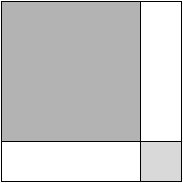
\includegraphics[scale=0.4]{FiguresMaths/proofa2plusb2}
\caption{A geometrical proof of the identity $(n+1)^2 = n^2 + 2n + 1$.}
       \label{fig:proofa2plusb2}
\end{center}
\end{figure}
The figure tells its tale by exhibiting four rectangles that make up
an $(n+1) \times (n+1)$ square; the area of this square is, of course,
$(n+1)^2$.  This large square is made up of four rectangles.
\begin{itemize}
\item
Reading across the top of the figure, we encounter a darkly shaded $n
\times n$ square (area $= n^2$) and an unshaded $n \times 1$ rectangle
(area $= n$).
\item
Reading across the bottom of the figure, we encounter an unshaded $1
\times n$ rectangle (area $= n$) and a lightly shaded $1 \times 1$
square (area = $1$).
\end{itemize}
The overall message is that $(n+1)^2$ (the area of the large,
composite, square)

\begin{tabular}{ll}
is the sum of & \\
  & $n^2$ (the area of the darkly shaded square) \\
plus & \\
  & $2n$ (the combined areas of the unshaded rectangles) \\
plus & \\
  & $1$ (the area of the lightly shaded square)
\end{tabular}
\medskip

Let now develop a more complex example.



\subsection{Fubini's principle}
\label{sec:Fubini}

\index{Fubini, Guido}

\subsubsection{The proof technique}

The previous technique is also called a \textit{proof without words}
(sous-entendu: with the evidence of a graphical argument).
Here, we use a slightly different idea while representing natural numbers as a set of objects (bullets).

The principle is to count the objects in two different ways, one being straightforward.
Changing the representation obviously does not change the value
since there is a one-to-one correspondence.


\subsubsection{Sample proofs: Computing the sum of the $n$ first integers}




\subsection{Combinatorial Proofs}

We introduce here a less conventional type of proofs that look at a result
as counting using combinatorial arguments.
This is illustrated by the previous example of computing the sum of the $n$ first integers:
\[ 1+2+ \ldots + n \ = \ {n \choose 2}.  \]
Choosing $2$ elements among $n$ can be done by choosing the last element (say at index $k$)
{\Denis k starts at 2 and goes to n}
and then, choosing the other one among the $k-1$ remaining ones before $k$, 
which can be mathematically written as:
\[ \ {n \choose 2} \ = \  \sum_{k=2}^n  \ {k-1 \choose 1} \ = \  \sum_{k=2}^n  (k-1) \ = \  \sum_{k=1}^{n-1}  k \ = \ \frac{(n)(n-1)}{2}\]



\subsection{Proof by computer}

Include here a brief presentation of the proof by computer, tell the story of 
the 4-color theorem.

%\subsection{Analyses via Linear Recurrences}
%\label{sec:linear-recurrences-1}
%
%\begin{theorem}[The Master Theorem for Linear Recurrences]
%\label{thm:master-thm-1}
%\index{The Master Theorem for Linear Recurrences}
%Let the function $F$ be specified by the following linear recurrence.
%\begin{equation}
%\label{eq:Lin-Recur:start-1}
%F(n) \ = \ \left\{
%\begin{array}{cl}
%a F(n/b) + c & \mbox{for } n \geq b \\
%c & \mbox{for } n < b
%\end{array}
%\right.
%\end{equation}
%Then the value of $F$ on any argument $n$ is given by
%\begin{equation}
%\label{eq:Lin-Recur:solve-1}
%\begin{array}{lclll}
%F(n) & = & (1 + \log_b n)c &  & \mbox{if } a=1 \\
%     &   &                 &  & \\
%     & = &
%  {\displaystyle
%  \frac{1-a^{\log_b n}}{1-a} \ \approx \ \frac{1}{1-a}
%  }
% &  & \mbox{if } a<1 \\
%    &   &                  & & \\
%    & = &
%  {\displaystyle
%\frac{a^{\log_b n} -1}{a-1}
%  }
% & & \mbox{if } a>1
%\end{array}
%\end{equation}
%\end{theorem}
%
%


